\documentclass[11pt, a4paper,oneside]{book}

\usepackage{caption}
\usepackage{a4wide}
\usepackage{makeidx}
\usepackage{float}
\usepackage{listings}
\usepackage{color}
\usepackage{textcomp}
\usepackage{alltt}
\usepackage{amsmath}
\usepackage{times}
\usepackage{ifpdf}
\usepackage{graphicx}
\usepackage{color} %colors in text
\usepackage{textcomp} % 
\usepackage[T1]{pbsi} %hand writting nice 
\usepackage[T1]{fontenc} %more fonts
\usepackage{mathrsfs} % letters for math
\usepackage{amsmath} % math formulas
\usepackage[all]{xy} % for drawing
\usepackage{listings}
\usepackage{amssymb}
%\usepackage[parfill]{parskip}
\definecolor{gray}{rgb}{0.7,0.7,0.7} 
\usepackage{enumerate} %for enumerate
\usepackage{subfigure}
\usepackage{epsfig}
\usepackage{float}
\usepackage{algorithm}
\usepackage[noend]{algorithmic}
\usepackage[dvipdfm]{hyperref}
\usepackage{multicol}
\usepackage{sectsty}
\usepackage{multirow}
%\ifpdf
%\usepackage[pdftex,
%            pagebackref=true,
%            colorlinks=true,
%            linkcolor=blue,
%            unicode
%           ]{hyperref}
%\else
%\usepackage[ps2pdf,
%            pagebackref=true,
%            colorlinks=true,
%            linkcolor=blue,
%            unicode
%           ]{hyperref}
%\usepackage{pspicture}
%\fi
\usepackage[utf8]{inputenc}
\makeindex
\setcounter{tocdepth}{3}
%\usepackage[light,condensed,math]{kurier}
%\renewcommand{\thechapter}{\Roman{chapter}}
%DEFINE NEW COMMANDS_________________________________________________________
%\newcommand{\clearemptydoublepage}{%
%  \newpage{\pagestyle{empty}\cleardoublepage}%
%}
\newcommand{\ds}{\displaystyle}
\newcommand{\todo}[1]{\textcolor{red}{\textbf{#1}}}
\newcommand{\fade}[1]{\textcolor{gray}{\textbf{#1}}}
\newcommand{\myemph}[1]{{\normalfont\emph{#1}}}
\newcommand{\tit}{\textit}

\usepackage[left=4cm, right=4cm, top=4cm, bottom=4cm]{geometry}
%____________________________________________________________________________
\begin{document}
	%THE TITLE PAGE & STUFF_________________________________________________________________
	%\fontfamily{arial}\selectfont
	%\fontfamily{courier-ttf}\selectfont
	%\fontfamily{comicsans}\selectfont
	%\fontfamily{franklingothic}\selectfont
	%\fontfamily{impact}\selectfont Impact
	%\fontfamily{palatino-ttf}\selectfont
	%\fontfamily{sylfaen}\selectfont 
	%\fontfamily{tahoma}\selectfont
	%\fontfamily{times-ttf}\selectfont 
	%\fontfamily{trebuchet}\selectfont 
	%\fontfamily{verdana}\selectfont 
	\fontfamily{georgia}\selectfont\normalsize

	\hypersetup{pageanchor=false}
	\begin{titlepage}
	\begin{figure}[!hbtp]
		\begin{flushright}
			
\epsfig{file=images/uva.eps, width=0.3\linewidth}
		\end{flushright}
	\end{figure}
	\vspace*{2cm}
	\begin{center}
	\rule{\linewidth}{1px}\\[10pt]
	\Huge{Texture Synthesis for Material Classification}
	\rule{\linewidth}{1px}\\[10pt]
	\vspace*{1cm}
	\large{Master\rq s Thesis in Artificial Intelligence -- Intelligent Systems}
	\large
	\vspace*{4cm}
	\begin{multicols}{2}
		\begin{flushleft}
			{\emph{Author:}\\
			Jasper van Turnhout\\
			\textit{jturnhou@science.uva.nl}\\ 
			Student number: 0312649}  
		\end{flushleft}
		\begin{flushleft}
			{\emph{Supervisors:}\\
			\href{mailto:Th.Gevers@uva.nl}{Prof. dr. Theo Gevers}\\
			\href{mailto:geusebroekuva.nl}{Dr. Jan-Mark Geusebroek}\\
			Informatics Institute, Faculty of Science, University of Amsterdam\\
			}
		\end{flushleft}
	\end{multicols}
	\end{center}
	\vspace*{6cm}
	\end{titlepage}
	%ABSTRACT PAGE____________________________________________________________________________
	\thispagestyle{empty}
	\section*{Abstract}
		In this research, the problem of material classification is addressed. Previous research shows how one can derive features based on Gaussian filter responses from material images and obtain high classification accuracies using simple classifiers such as Nearest Neighbor or Bayes. To model the appearance of material under different illumination conditions a lot of data is needed to obtain satisfactory models. This rises the need for novel data recorded under controlled conditions, which is an intensive task. Rather than recording this novel data, one could synthesize this data using albedo and surface normal recovery from present data. In previous research it has been shown that synthesis using simple Lambertian reflectance results in good accuracy when compared to the real data. In this research, synthesized data is compared in terms of classification accuracy for more complex reflectance models with respect to Lambertian reflectance. Small significant improvements have been reported for the more complex reflectance models, and suggests that future work needs better methods for the recovery of the albedo and surface normals.


	%CONTENT PAGE____________________________________________________________________________
	\newpage
	\pagenumbering{roman}
	\tableofcontents
	%CHAPTERS & SUB-CHAPTERS____________________________________________________________________
	\newpage
	\pagenumbering{arabic}
	\hypersetup{pageanchor=true}
	\chapter{Introduction}
	\hypertarget{Introduction}{
}

For human perception, recognizing materials is a very important aspect in our visual system. We can do this flawlessly for a great number of different materials. As a human, we can easily determine whether a surface is smooth, rough, soft or hard by just looking at it. We are also capable of recognizing  materials under great variety of visual conditions. For example, when observing a car from an arbitrary point of view, we always perceive the surface of the car differently when considering the light reflected on the metallic surface which differs from viewpoint to viewpoint. Yet, we have no problem in classifying this surface as metal. The same accounts for many other materials we perceive on a daily base.

Material recognition is a field of research in computer vision with the goal to develop classification systems that can identify various material categories observed in daily life. Examples of such categories are metal, wood, fabric, plastic and glass. Material recognition differs and should not be confused with object recognition and texture recognition. This difference is illustrated in figure \ref{fig:ObjectRecognition} and \ref{fig:TextureRecognition}. A system capable of recognizing materials can greatly enhance the performance of object recognition or scene recognition.

Research has been done on several different material databases and good recognition accuracies have been reported. However, there are suggestions that the accuracies reported are all database dependent \cite{ExploringFeatures} since none of these databases could possibly capture the large variation in appearance of material classes. The large variation of a material class is also addressed as the intra-class variation. 

In this research, we investigate how realistic image synthesis can be employed to create synthetic image data for various material classes. With the aid of image synthesis it is possible to generate infinite amounts of data with arbitrary viewpoint and illumination conditions. This makes it possible to create image data that is not present in material databases, thus making it possible to increase the intra-class variation of material classes.

This chapter gives a short introduction to the problem of material recognition and how image synthesis can be applied to improve recognition performance.

\begin{figure}[htbp!]
	\begin{center}
		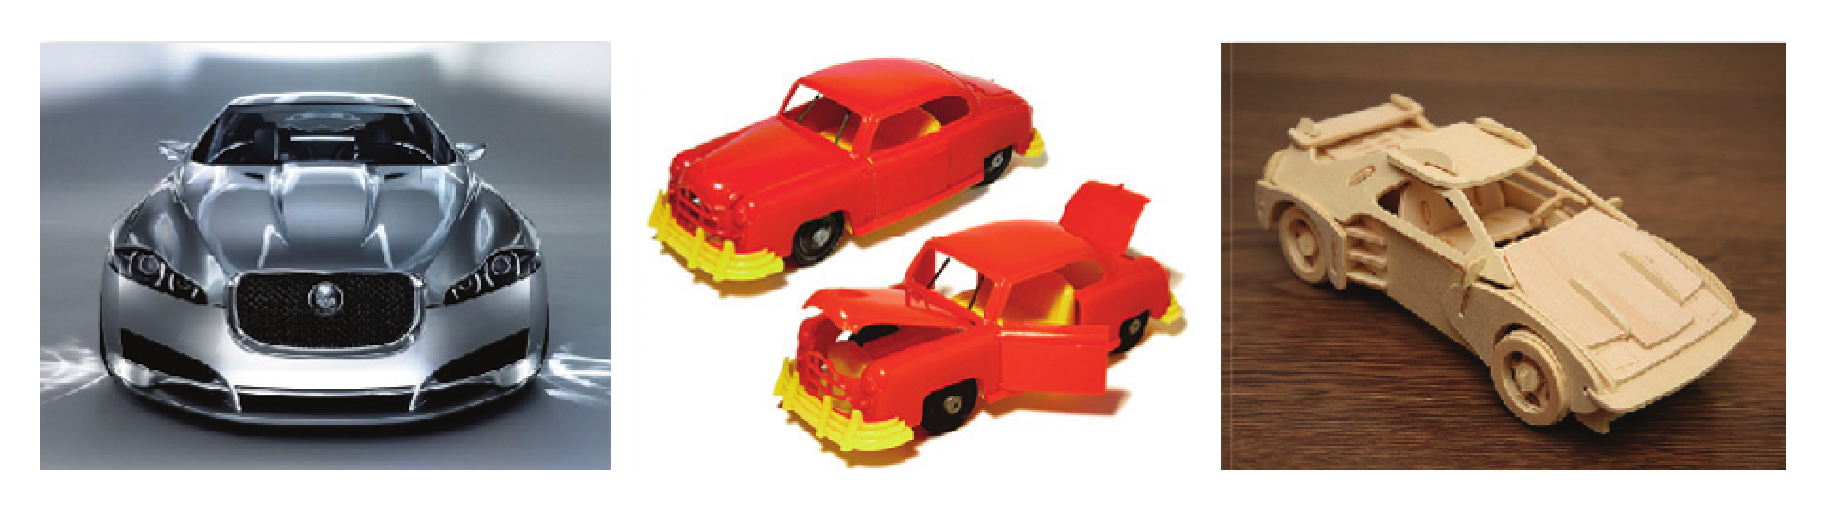
\epsfig{file=images/ObjectRecognition.eps, width=0.6\linewidth}
	\end{center}
	\caption{{\it Object recognition and material recognition: all three pictures depict the same object. However, they are made from metal, plastic and wood respectively. Image adapted from \cite{ExploringFeatures}.}}
	\label{fig:ObjectRecognition}
\end{figure}

\begin{figure}[htbp!]
	\begin{center}
		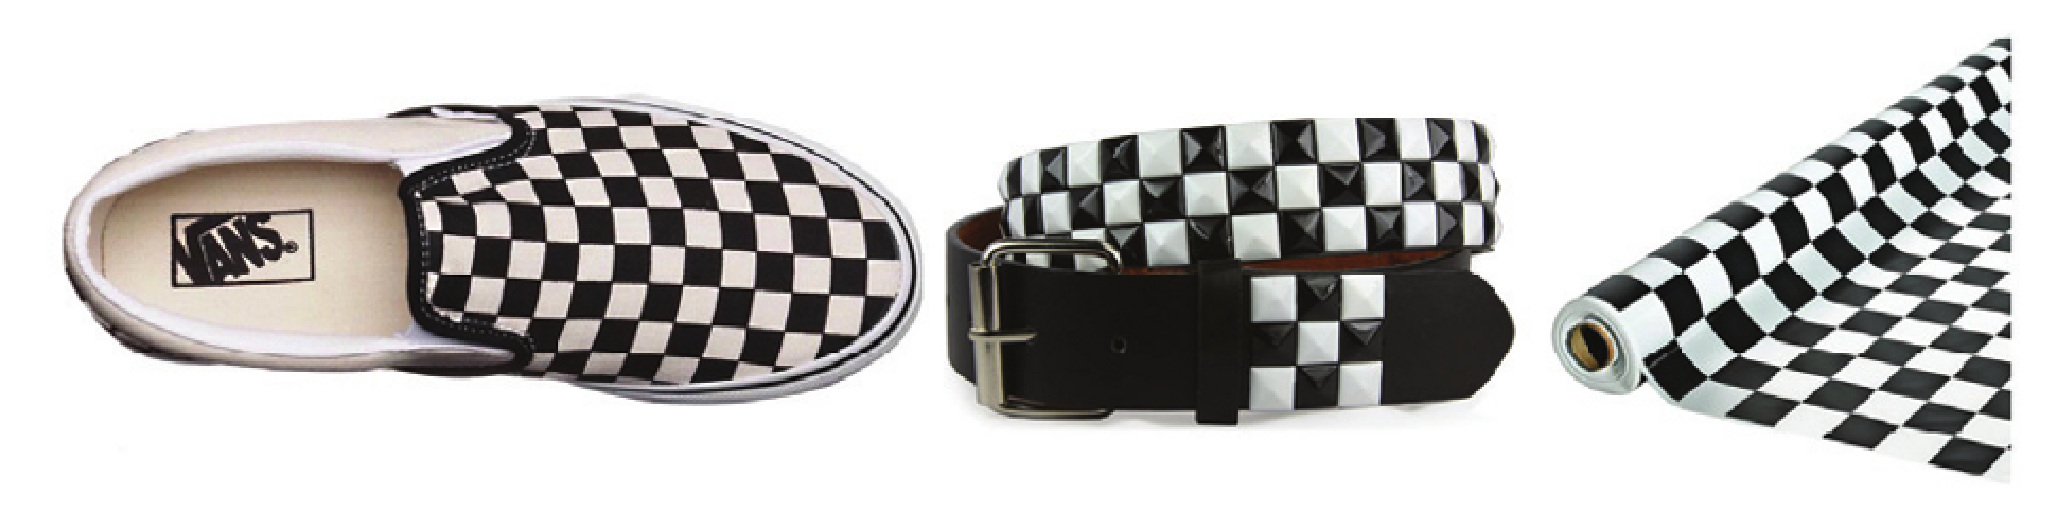
\epsfig{file=images/TextureRecognition.eps, width=0.6\linewidth}
	\end{center}
	\caption{{\it Texture recognition and material recognition: all three pictures depict the same pattern. However, they are made from fabric, plastic and paper respectively. Image adapted from \cite{ExploringFeatures}.}}
	\label{fig:TextureRecognition}
\end{figure}

\section{Material Recognition}
Material recognition is defined as the task to correctly classify a novel image from a material surface. When building a system for material recognition, prediction of a material class is done preferably on a single image of a material surface. This creates a difficult task as the variation in appearances of materials is considerably enhanced by illumination differences or arbitrary viewpoints. Some examples of how much a surface can vary are shown in figure \ref{fig:PhoTexExamples}.

In recent research, material databases have been created containing various illumination and viewpoint conditions that try to capture the large variety within each  material class. The difficulty is to obtain robust features from the image data that covers various occurrences of materials with different spatial properties as well as distinct illumination properties. 

\begin{figure}[htbp!]
	\begin{center}
		\subfigure[aab]{\epsfig{file=images/examples/0.aab.0.30.0.eps, width=0.15\linewidth}}\label{fig:aab1}
		\subfigure[acd]{\epsfig{file=images/examples/1.acd.0.30.0.eps, width=0.15\linewidth}}\label{fig:acd1}
		\subfigure[adh]{\epsfig{file=images/examples/2.adh.0.30.0.eps, width=0.15\linewidth}}\label{fig:adh1}

		\subfigure[aab]{\epsfig{file=images/examples/0.aab.0.75.180.eps, width=0.15\linewidth}}\label{fig:aab2}
		\subfigure[acd]{\epsfig{file=images/examples/1.acd.0.75.180.eps, width=0.15\linewidth}}\label{fig:acd2}
		\subfigure[adh]{\epsfig{file=images/examples/2.adh.0.75.180.eps, width=0.15\linewidth}}\label{fig:adh2}
	\end{center}
	\caption{{\it Example images from the PhoTex database. The upper row is recorded under a slant of $30^0$ and a tilt of $0^o$. The lower row is recorded under a slant of $75^0$ and a tilt of $180^0$. The captions are the material labels.}}
	\label{fig:PhoTexExamples}
\end{figure}

The {\it CuRET} database captures such properties for 60 different material classes with each over 200 different illumination and viewing directions. This database has been used in the development of texton descriptors to capture the various material properties. In later research on the {\it CuRET} database, parametric models have been developed to deal with the limits of a texton dictionary. The {\it ALOT} and {\it PhoTex} databases have been used in more physically-based computer vision experiments where the geometrical structure of the surface is used for development of robust descriptors. In all these experiments, classification rates of 95\% and higher are reported using various methods such as Naive Bayes, Nearest Neighbor and Support Vector Machines.

The reported classification rates are of great accuracies in general, it seems that most of the difficulties have been solved for material recognition. However, the suggestion that the databases do not capture the intra-class variety for the material classes poses the problem of data shortage. Recording the data is a time-consuming task and will not be sufficiently diverse to capture all possible illumination and viewing directions. 

\section{Image Synthesis}
The field of computer graphics has accomplished imagery of great realism over the past few decades. With increasing computational power, it became possible to synthesize realistic images using expensive physically-based light simulations. 

Various models have been developed for the synthesis of diffuse, glossy or shiny materials. These models use as input for per-pixel generation of an image a surface normal, the surface albedo, a viewing direction, an illumination direction and illumination properties such as the color of the light source. With proper reconstruction of the surface normals and surface albedo for a material, it is possible to generate an infinite amount of data with arbitrary viewing and illumination directions. Databases such as {\it PhoTex} and {\it ALOT} were created with physically-based computer vision in mind. With image data available for each material class with recorded light source directions, it is possible to recover surface normals and surface albedo for material classes. 

In research done by Targhi \cite{Targhi}, the synthesis of material images has been used to augment training-sets to a point of saturation where perfect predictions were made \cite{Targhi}. For the synthesis of image data, the Lambertian reflection model was used. This reflection model is limited to the synthesis of purely diffuse materials only, since the reflection model does not simulate illumination phenomena such as speculars which are observed on glossy and shiny surfaces. Other reflection models should be considered as well if we want to be able to synthesize images for other than purely diffuse materials.

\section{Goal of this thesis}
In this research, the aim is to investigate the addition of more sophisticated reflection models for the synthesis of realistic image data. We research and implement combinations of Lambertian reflectance with models for speculars such as Phong, Blinn-Phong and Torrance-Sparrow, as well as a more sophisticated model for diffuse reflection. 

The synthetic image data is used for training models for material classification. These models are tested against two datasets: a dataset consisting of mainly diffuse materials and a dataset consisting of shiny/glossy materials. Our main focus is to test and compare performance of classification when using only synthetic image data for training the models for classification. With the addition of specular reflection models for synthesis, we can expect some improved models when comparing the performance with models obtained from synthetic data using Lambertian reflection only.

\section{Overview of this thesis}
In the next chapter, some of the state-of-the-art methods and their experiments are outlined. Some of these methods are adapted for the experiments in this research. Chapter 3 outlines some fundamentals that are used for understanding local reflection models. In chapter 4 the methods and data that we adapt in this research will be discussed in more detail. In chapter 5, a set of empirical reflection models that we implemented for the experiments are discussed in detail. In chapter 6, a set of more physical-based reflection models that we implemented are discussed in detail. In chapter 7, the experiments and their results are reported and the last chapter holds the conclusion and future works.


	\chapter{Related work}
	\hypertarget{RelatedWork}{
\section{Varma \& Zisserman}\label{VarmaZisserman}
%\label{Textons}\index{Textons@{Texton Dictionary}}}
}

In earlier research on the topic of material recognition, a lot of focus was on the albedo variation on top of a flat surface. More recently, this focus has shifted towards surface normals, which cause the 3D effects we perceive. Photometric stereo based classification algorithms have been developed to capture these features.
The need for larger texture databases that captures the variety in viewpoint and illumination resulted in the creation of the CUReT database (Dana et al, 1999). Dana and Nayar developed parametric models based on surface roughness and correlation lenghts which were tested against the CUReT database. However, in their research, no significant results were reported.

Leung and Malik (2001) were the first to introduce the texton modeling method...

\begin{itemize}
	\item{CUReT Database}
	\item{Texton Dictionary}
	\item{Filter banks (LM, MR8, Schmid)}
	\item{Chi-squared distance}
	\item{Nearest Neighbour classifier}
\end{itemize}

\section{Broadhurst}\label{Broadhurst}
\begin{itemize}
	\item{CUReT Database}
	\item{eqi-count histograms}
	\item{MR8 filter bank}
	\item{Mallow distance}
	\item{multivariate Gaussian classifier}
\end{itemize}


In his article, Broadhurst presents a parametric approach to estimate the likelihood of homogeneously textured images. His work extends the framework proposed by Levina (PhD thesis, 2002) by using a Gaussian Bayes classifier instead of a 1-NN classifier. To model each texture class, he uses multivariate Gaussian distributions to model the intra-class variability of each marginal histogram. This is done by mapping the joint marginal histograms into Euclidean space and applying PCA [to obtain the eigenvalues and expected projection error for each class].
Marginal distributions of each filter response are estimated by using non-parametric histograms. There are several advantages to this:
	1.This approach eliminates effectively the need to use a texton dictionary as proposed by Varma \& Zisserman (2004). The use of such dictionary would limit the generalization of a texture class and also needs clustering in high-dimensional spaces.
	2. Marginal distributions can be estimated accurately, while joint distributions often suffer from the curse of dimensionality.
Although less descriptive than joint conditional distributions, the dependencies among filter responses are captured by estimating the joint intra-class variation of the marginals. This approach increases the descriptive power of the marginal distributions while still maintaining the computational efficiency. The method is applied to the MR8 filter bank (described in Varma \& Zisserman).

In order to perform statistical analysis on the marginal distributions, the distributions are mapped to points in Euclidean space. 
Responses are represented as marginal histograms [as described in another paper, look this up]. The Mallow Distance is used to measure distribution similarity in the Euclidean space. The Mallow Distance used for comparing two continuous one-dimensional distributions is given by [insert formula]. To compare discrete distributions, consider two equi-count histograms x and y with n bins and the average value of each bin stored. Consider these values sorted in order [n values are sorted]. x and y can be represented as vectors x and y. The Mallows distance between these vectors is given by: [insert formula]. The described representation maps histograms to points in Euclidean space with distances corresponding to M2 histogram distances.

Experiments are run on samples from the CUReT database, which consists of 61 texture classes with each 205 different viewing and illumination conditions. Each class experiences 3D effect such as interreflections, speculars and shadowing, which gives a large intra-class variability, but the database is sparse in its rotation and scaling conditions. In a preprocessing step, the images are converted to gray-scale and are processed to have zero-mean and unit-variance to get intensity invariance. The MR8 filter bank is used to gain rotationally invariant features by using the maximum responses over the orientations.
Levinka has developed a framework for classification using filter banks, marginal histograms, the Mallow distance and a 1NN classifier. The 1-NN classifier requires a distance measure between two sets of marginal distributions. Broadhurst defines this to be the product of the M2 marginal distances described in section 2. The variation of marginal distributions can be measured jointly or independently. A joint 1-NN classifier measures the distance between a target image and all the training images as the distance between each set of marginals. The target image is then classified using the closest training image. For an independent 1-NN classifier, the minimum M2 distance between each target marginal and each class is computed. The total distance to a class is defined as the product of each minimum marginal distance.



4. Gaussian Bayes Classification

(skip the Markov Random Field parts as they are not in the scope of the thesis)

\section{Targhi}\label{Targhi}
\begin{itemize}
	\item{PhoTex database}
	\item{ALOT database}
	\item{Photometric Stereo}
	\item{Lambertian reflection}
	\item{Broadhurst experiment}
\end{itemize}

\section{Reflection Models}
\begin{itemize}
	\item{Lambertian}
	\item{Phong, Blinn-Phong}
	\item{Ward}
	\item{Lafortune}
	\item{Microfacets}
	\item{Cook-Torrance}
	\item{Oren-Nayar}
\end{itemize}

	\chapter{Approach}
	\hypertarget{Approach}{
\section{Photometric Stereo}\label{PhotometricStereo}
}

\begin{itemize}
	\item{core formula}
	\item{Lambertian assumption}
\end{itemize}


\section{Classification}
\begin{itemize}
	\item{multivariate Gaussian Classifier, Mallow distance}
	\item{Texton Dictionary, Chi-distance}
\end{itemize}


	\chapter{Fundamentals}
	\hypertarget{Fundamentals}{
}

In this chapter, some fundamental properties of local illumination models will be outlined. Although these fundaments are 

\section{BRDF}
The bi-directional reflectance distribution function, first described by {\it Nicodemus et al} \cite{Nicodemus}, can be used as a tool for describing the scattering of light from a surface. This function is assumed to be a local illumination model, meaning that incoming light will be reflected at the point of intersection with the surface \footnote{The BRDF is an approximation of the BSSRDF (Bi-directional scattering surface reflectance distribution function). The BSSRDF simulates the phenomenon of subsurface scattering; light enters the material and after scattering leaves the material at a point different from the intersection point of the incoming light beam.}

\section{Lambert's Cosine Law}

	\chapter{Empirical Models}
	\hypertarget{empiricalModels}{
}

%\begin{itemize}
%	\item{Lambertian}
%	\item{Phong, Blinn-Phong}
%	\item{Ward}
%	\item{Lafortune}
%\end{itemize}

\noindent For the texture synthesis of the materials, various local reflection \footnote[1]{Another set of reflection models are global illumination models. These are beyond the scope of this thesis.} models can be used. This chapter will outline the empirical models used in the process of texture synthesis. These models capture reflectance behaviour using mathematical models without using any basic laws of physics. Such models are widely used for their simplicity and because they can be controlled by setting only a small set of parameters to obtain desired results.

\section{Lambertian reflectance}\label{Lambertian}
	One of the most used empirical models is Lambertian reflectance. In computer graphics, this model is mainly used to model diffuse reflectance. Surfaces with such properties appear equally bright from all viewing angles because the light is reflected with equal intensity in all directions. The brightness of the surface is only dependent of the angle $\theta$ between the surface normal $\vec{\mathbf{n}}$ and the light source direction $\vec{\mathbf{l}}$ as shown in figure X. We can look at a diffuse surface on microscopic level to understand how this works. 

If we look at \ref{fig:BEAM}, we can see how an incoming light beam projects a differential area $dA$ on the surface. If the surface normal and the light direction are parallel and in the same direction as shown in figure \ref{fig:BEAM}, the energy the area receives and reflects is proportional to $dA$. If the beam is projected on the surface such that it covers a larger area as shown in \ref{fig:BEAM}, the amount of energy reflected from area $dA$ is proportional to $\cos \theta$. The amount of energy reflected per unit area is less on surface 2 compared to surface 1 since the beam covers a larger area. This observation of radiance behaviour is also known as Lambert's Cosine Law. In general, for Lambertian reflectance, the amount of light observed by the viewer is indepenendent of the viewing angle, and is only dependent on the angle of the incidence of the light source. The full equation is given by:

		\begin{eqnarray*}
			I = I_pk_d\cos\theta
		\end{eqnarray*}

Here, $I$ is the reflected amount of light, $I_p$ is the intensity of the light source, $k_d$ is the \tit{diffuse reflection coefficient} which varies between 0 and 1 and is material dependent. The cosine term is defined between $0^0$ and $90^0$. This means that the surface is treated as self-occluding; angles outside this range will result in negative values for the cosine term and are treated as a $max({0,\cos\theta})$, resulting in zero intensity falling on the surface. If both $\vec{\mathbf{n}}$ and $\vec{\mathbf{l}}$ are normalized, we can write the equation as:

		\begin{eqnarray*}
			I = I_pk_d(\vec{\mathbf{n}} \cdot \vec{\mathbf{l}})
		\end{eqnarray*}

This model is used effectively for the synthesis of diffuse surfaces and in interactive software since the reflection term doesn't need to be recomputed whenever the view changes. However, most materials are deviating from Lambertian for angles of view or incidence greater than $60^0$ \cite{DigitalModeling}. Another shortcoming of Lambertian reflectance is that it does not include the observation of speculars on materials. For these reasons the model is insufficient to synthesize materials with a more glossy nature since they will need the speculars to be present. 


\begin{figure}[H]
	\begin{center}
		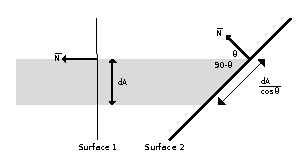
\epsfig{file=images/beam_example.eps, width=0.5\linewidth}
	\end{center}
	\caption{Beam shown in gray, projecting an area on surfaces. The projected area on surface 1 equals $dA$, and on surface 2 equals $\frac{dA}{\cos\theta}$. \tit{Image adapted from Computer Graphics, Principles and Practice \cite{ComputerGraphics}}}
	\label{fig:BEAM}
\end{figure}




	\section{Phong Reflectance}\label{Phong}
		With the Lambertian assumption of light reflecting equally into all direction, we can expect poor quality synthesis when we're dealing with more glossy/specular surfaces such as metallic, stone and plastic materials. As Bui-Tuong Phong wrote in his article, if the goal in shading a computer-synthesized image is to simulate a real physical object, then the shading model should in some way imitate real physical shading situations \cite{Phong}. Phong reflectance is a popular model, based on the empirical observation of how shiny surfaces can have small specular highlights, and how these observed speculars are related to the view direction of the observer.
The general idea of Phong reflection is shown in figure \ref{fig:SPECULAR1}. Here we have an incident angle $\theta_i$ and an equal reflection angle $\theta_r$. The angle between $\vec{\mathbf{r}}$ and $\vec{\mathbf{v}}$, $\alpha$, defines how strong a specular is perceived by the observer. If this angle is zero (ie. the reflection- and view-direction are in the same direction), the perceived intensity will be maximal. When this angle increases, the observed intensity of the specular will fall off fast.

\begin{figure}[H]
	\begin{center}
		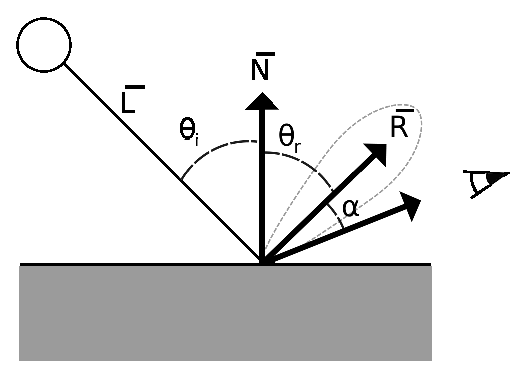
\epsfig{file=images/specular_reflection.eps, width=0.4\linewidth}
	\end{center}
	\caption{Specular reflection. $\theta_i$ is the angle of the incoming light, and is equal to the reflected angle $\theta_r$. $\alpha$ is the angle between the view direction and the reflected light.}
	\label{fig:SPECULAR1}
\end{figure}


\noindent The reflection model is computed as:

	\begin{eqnarray*}
		I = i_a + k_d(\vec{\mathbf{l}} \cdot \vec{\mathbf{n}}) + k_s(\vec{\mathbf{r}} \cdot \vec{\mathbf{v}})^\alpha
	\end{eqnarray*}

\begin{itemize}
	\item[] $i_a$ is a parameter controlling the ambient lighting.
	\item[] $k_d$ is the diffuse reflection coefficient.
	\item[] $k_s$ is the specular reflection coefficient.
	\item[] $\vec{\mathbf{l}}$ is the direction vector for the light source.
	\item[] $\vec{\mathbf{v}}$ is the direction vector for the observer.
	\item[] $\vec{\mathbf{n}}$ is the surface normal.
	\item[] $\vec{\mathbf{r}}$ is the direction vector for the reflected light, 
		calculated as $2\vec{\mathbf{n}}(\vec{\mathbf{l}} \cdot \vec{\mathbf{n}}) - \vec{\mathbf{l}}$
	\item[] $\alpha$ is a parameter controlling the specular size, also known as the shininess constant, which is material-dependent. The greater $\alpha$ is, the smaller the size of the specular.
\end{itemize}

Here, the parameterse $k_d$ and $k_s$ are constants for diffuse and specular reflection respectively. 
This formula is simplified such that it doesn't involve more than one light source. More light sources could be incorporated easily by computing the diffuse and specular components for each light source separately and summing these to obtain the total contribution. With respect to the experiments, multiple light sources are not necessary. Also, the components defining colors are left out since we're only concerned about grayscale images in the experiments. The ambient term can be left out as well, since a preprocessing step will make the synthesized images intensity-invariant. A common complaint about the Phong model is that it is completely emperical, and doesn't abide the most basic law in physics - the conservation of energy. Appropriate normalization factors could be applied to constrain the model to this law.

	\section{Blinn-Phong Reflectance}\label{BlinnPhong}
		Short after Phong published his model, Blinn proposed an alternative to compute the specular component where the angle $\theta_s$, dot product between the reflection vector and viewing vector, could be replaced by $\theta_h$ \cite{Blinn}. This angle the dot product between the normal of the surface, and the so called halfway-vector $\vec{\mathbf{h}}$. This halfway-vector is the bivector between the light source vector $\vec{\mathbf{l}}$ and the view direction vector $\vec{\mathbf{v}}$, and is computed as:

	\begin{eqnarray*}
		\vec{\mathbf{h}} = \frac{\vec{\mathbf{l}} + \vec{\mathbf{v}}}{|\vec{\mathbf{l}} + \vec{\mathbf{v}}|}
	\end{eqnarray*}

He observed that mirror reflections only occur when the surface normal is aligned with the halfway-vector \cite{DigitalModeling}. When observing a material with glossy/shiny properties, the microscopic structure of the material is never entirely smooth and can be illustrated as microscopic small surfaces. The main normal of the surface is still $\vec{\mathbf{n}}$, but each micro-surface has its own surface normal as well. The distribution of the specular lobe can be expressed as the amount of microfacets with normals aligned with the halfway-vector, with a likelihood related to $\theta_h$.

Replacing $\theta_s$ with $\theta_h$ doesn't give the same reflectance function as with Phong reflection, and as a result it produces slightly different speculars. However, because of computational convenience, Blinn-Phong reflectance is being used in most systems these days.

	\chapter{Microfacet Models}
	\hypertarget{Physical Models}{
}

%\begin{itemize}
%	\item{Lambertian}
%	\item{Phong, Blinn-Phong}
%	\item{Ward}
%	\item{Lafortune}
%\end{itemize}

\noindent In the previous section, the reflection models were based on emperical observations, which result in non-perfect synthesis when applied. In this section, more complex reflection models for diffuse (and specular) reflection are outlined. These models are based on a roughness model, micro-facets, and were introduced by Torrance and Sparrow \cite{TorranceSparrow}.

\section{Oren-Nayar Reflectance}\label{OrenNayar}
A big deficiency in approximating the body reflectance under the Lambertian assumption is that its view independent. This results in inaccurate approximations for several real-world objects, as experiments have demonstrated on several rough diffuse surfaces such as plaster, sand and cloth \cite{OrenNayar}. To overcome this deficiency, M. Oren and S.K. Nayar propose a more general reflection model for diffuse surfaces \cite{OrenNayar}.

	\chapter{Experiments}
	\hypertarget{experiments}{
}

%\begin{itemize}
%	\item{Lambertian}
%	\item{Phong, Blinn-Phong}
%	\item{Ward}
%	\item{Lafortune}
%\end{itemize}

\section{Setup}\label{sec:Experiments}
\section{Results}\label{sec:Results}


	\chapter{Conclusion}
	\hypertarget{conclusion}{
}

In this research we investigated how to improve the quality of synthetic image data for material recognition. Recent material databases try to capture the intra-class variation of materials by using different illumination and viewpoint conditions, but the intra-class variation within the material classes is restricted to the database. This seriously limits the research field of material recognition, and manually recording an amount of data to capture the intra-class variation for any material class is a difficult and time-consuming task. However, the synthesis of novel image data could help to bridge the gap of data sparseness.

Previous research showed that using a simple model for photometric stereo to recover surface normals and surface albedo can be used to synthesize enough data to achieve perfect classification accuracy \cite{Targhi}. However, the model was limited to diffuse materials only since the image synthesis was performed with Lambertian reflectance. 

Recovered surface normals and surface albedo from photometric stereo can be used as input for various reflection models and these reflection models can be used to simulate BRDF beyond that of Lambertian reflectance. With this setup, image data for the problem of material recognition can be synthesized using arbitrary illumination and viewpoint conditions to simulate diffuse and glossy/shiny material properties, thus increasing the intra-class variety of material classes.

In our experiments, the different reflection models are tested on image quality in two experiments on two different datasets. The datasets are designed such that one consists mostly of diffuse materials and the other consists of specular materials. 

On the diffuse material dataset, significant improvements were observed using reflection models that obey basic physical laws. Phong reflectance performed similar or worse than Lambertian reflectance. The other specular reflection models implemented, Blinn-Phong and Cook-Torrance performed slightly better than Lambertian reflectance. These models share the concept of micro-facets and outperform Phong reflectance, suggesting that more physical based reflectance models are useful in this task of image synthesis. The Oren-Nayar reflection model gives mixed results, performing similar or better than the baseline.

On the glossy/shiny material dataset, no significant improvements were observed in the experiments. The accuracy for the synthetic data is significantly worse for the glossy/shiny material dataset than that of the diffuse material dataset, even though we try various models for specular simulation.

The problem in the setup of these experiments is that of the recovery of surface normals and surface albedo. The quality of these recoveries are directly dependent on the set of image data used in this process and the assumptions made by the photometric stereo method. The algorithm for photometric stereo uses the Lambertian assumption to estimate the surface albedo and surface normals, and for this reason outliers in image data such as speculars are treated as if they are part of the surface albedo. RANSAC or surface normal smoothing are not able to improve the surface normals and surface albedo recovery under the Lambertian assumption. This suggests that more complex methods for photometric stereo are needed that are not constrained to the assumption of Lambertian surfaces to improve the quality of recovery. With the current material databases available that allow for photometric stereo, this is a difficult problem since only intensity information is present. 

For future work, additional analysis of materials could be of use for better estimation of parameters, such as the refraction indices for Fresnel and surface roughness parameters for micro-facet models since finding these settings through optimization is computational expensive. The addition of color in material databases with photometric image data could improve the quality of the recovery of surface normals and surface albedo. Methods exists that use models other than the Lambertian assumption. These models are more robust to outliers such as speculars in the photometric image data. With improved surface normals and surface albedo, it is likely that the synthesized image data will improve in quality.

	%___________________________________________________________________________________________
 	\nocite{*}
	\bibliographystyle{plain}
	\bibliography{bibtex}
	\printindex
\end{document}

